\chapter{Successioni Numeriche}\label{successioni-numeriche}

\defn{Definizione Successione Numerica}{
Si chiama \textbf{successione numerica} una funzione con dominio in $\N$
\[
f: n \in \N \to f(n) \in \R
\]
Si utilizza la seguente notazione: $f(n)=a_{n}\to$ Termine generale della successione.
Una successione si indica o con il suo termine generale $a_{n}$ oppure $\{a_{n}\}_{n\in \N}$.
}

\ex{1: $\quad a_{n}=\frac{1}{n}$}
\[
a_{n}=\frac{1}{n} \quad \text{allora} \quad1, \frac{1}{2}, \frac{1}{3}, \frac{1}{4},\dots, \frac{1}{n}
\]

\ex{2: $\quad a_{n}=(-1)^n$}
\[
a_{n}=(-1)^n \to -1,1,-1,1,\dots
\]

\ex{3: $\quad a_n =n$}
\[
a_n =n \to 1,2,3,\dots
\]

\ex{4: $\quad a_{n}=\frac{(-1)^n}{n}$}
\[
a_{n}=\frac{(-1)^n}{n}=-1, \frac{1}{2}, -\frac{1}{3}, \frac{1}{4}, -\frac{1}{5}
\]

\ex{5: $\quad a_{n}=-n^2$}
\[
a_{n}=-n^2=-1,-4,-9,-16
\]

\ex{6: $\quad a_{n}=\arctan n$}

\ex{7: $\quad a_{n}=2^n$}
\[
a_{n}=2^n=1,2,4,8,16,32,64,\dots
\]

\ex{8: Formula per il perimetro di un poligono inscritto}\label{perim-pol-inscritto}
\begin{figure}[H]
    \centering
    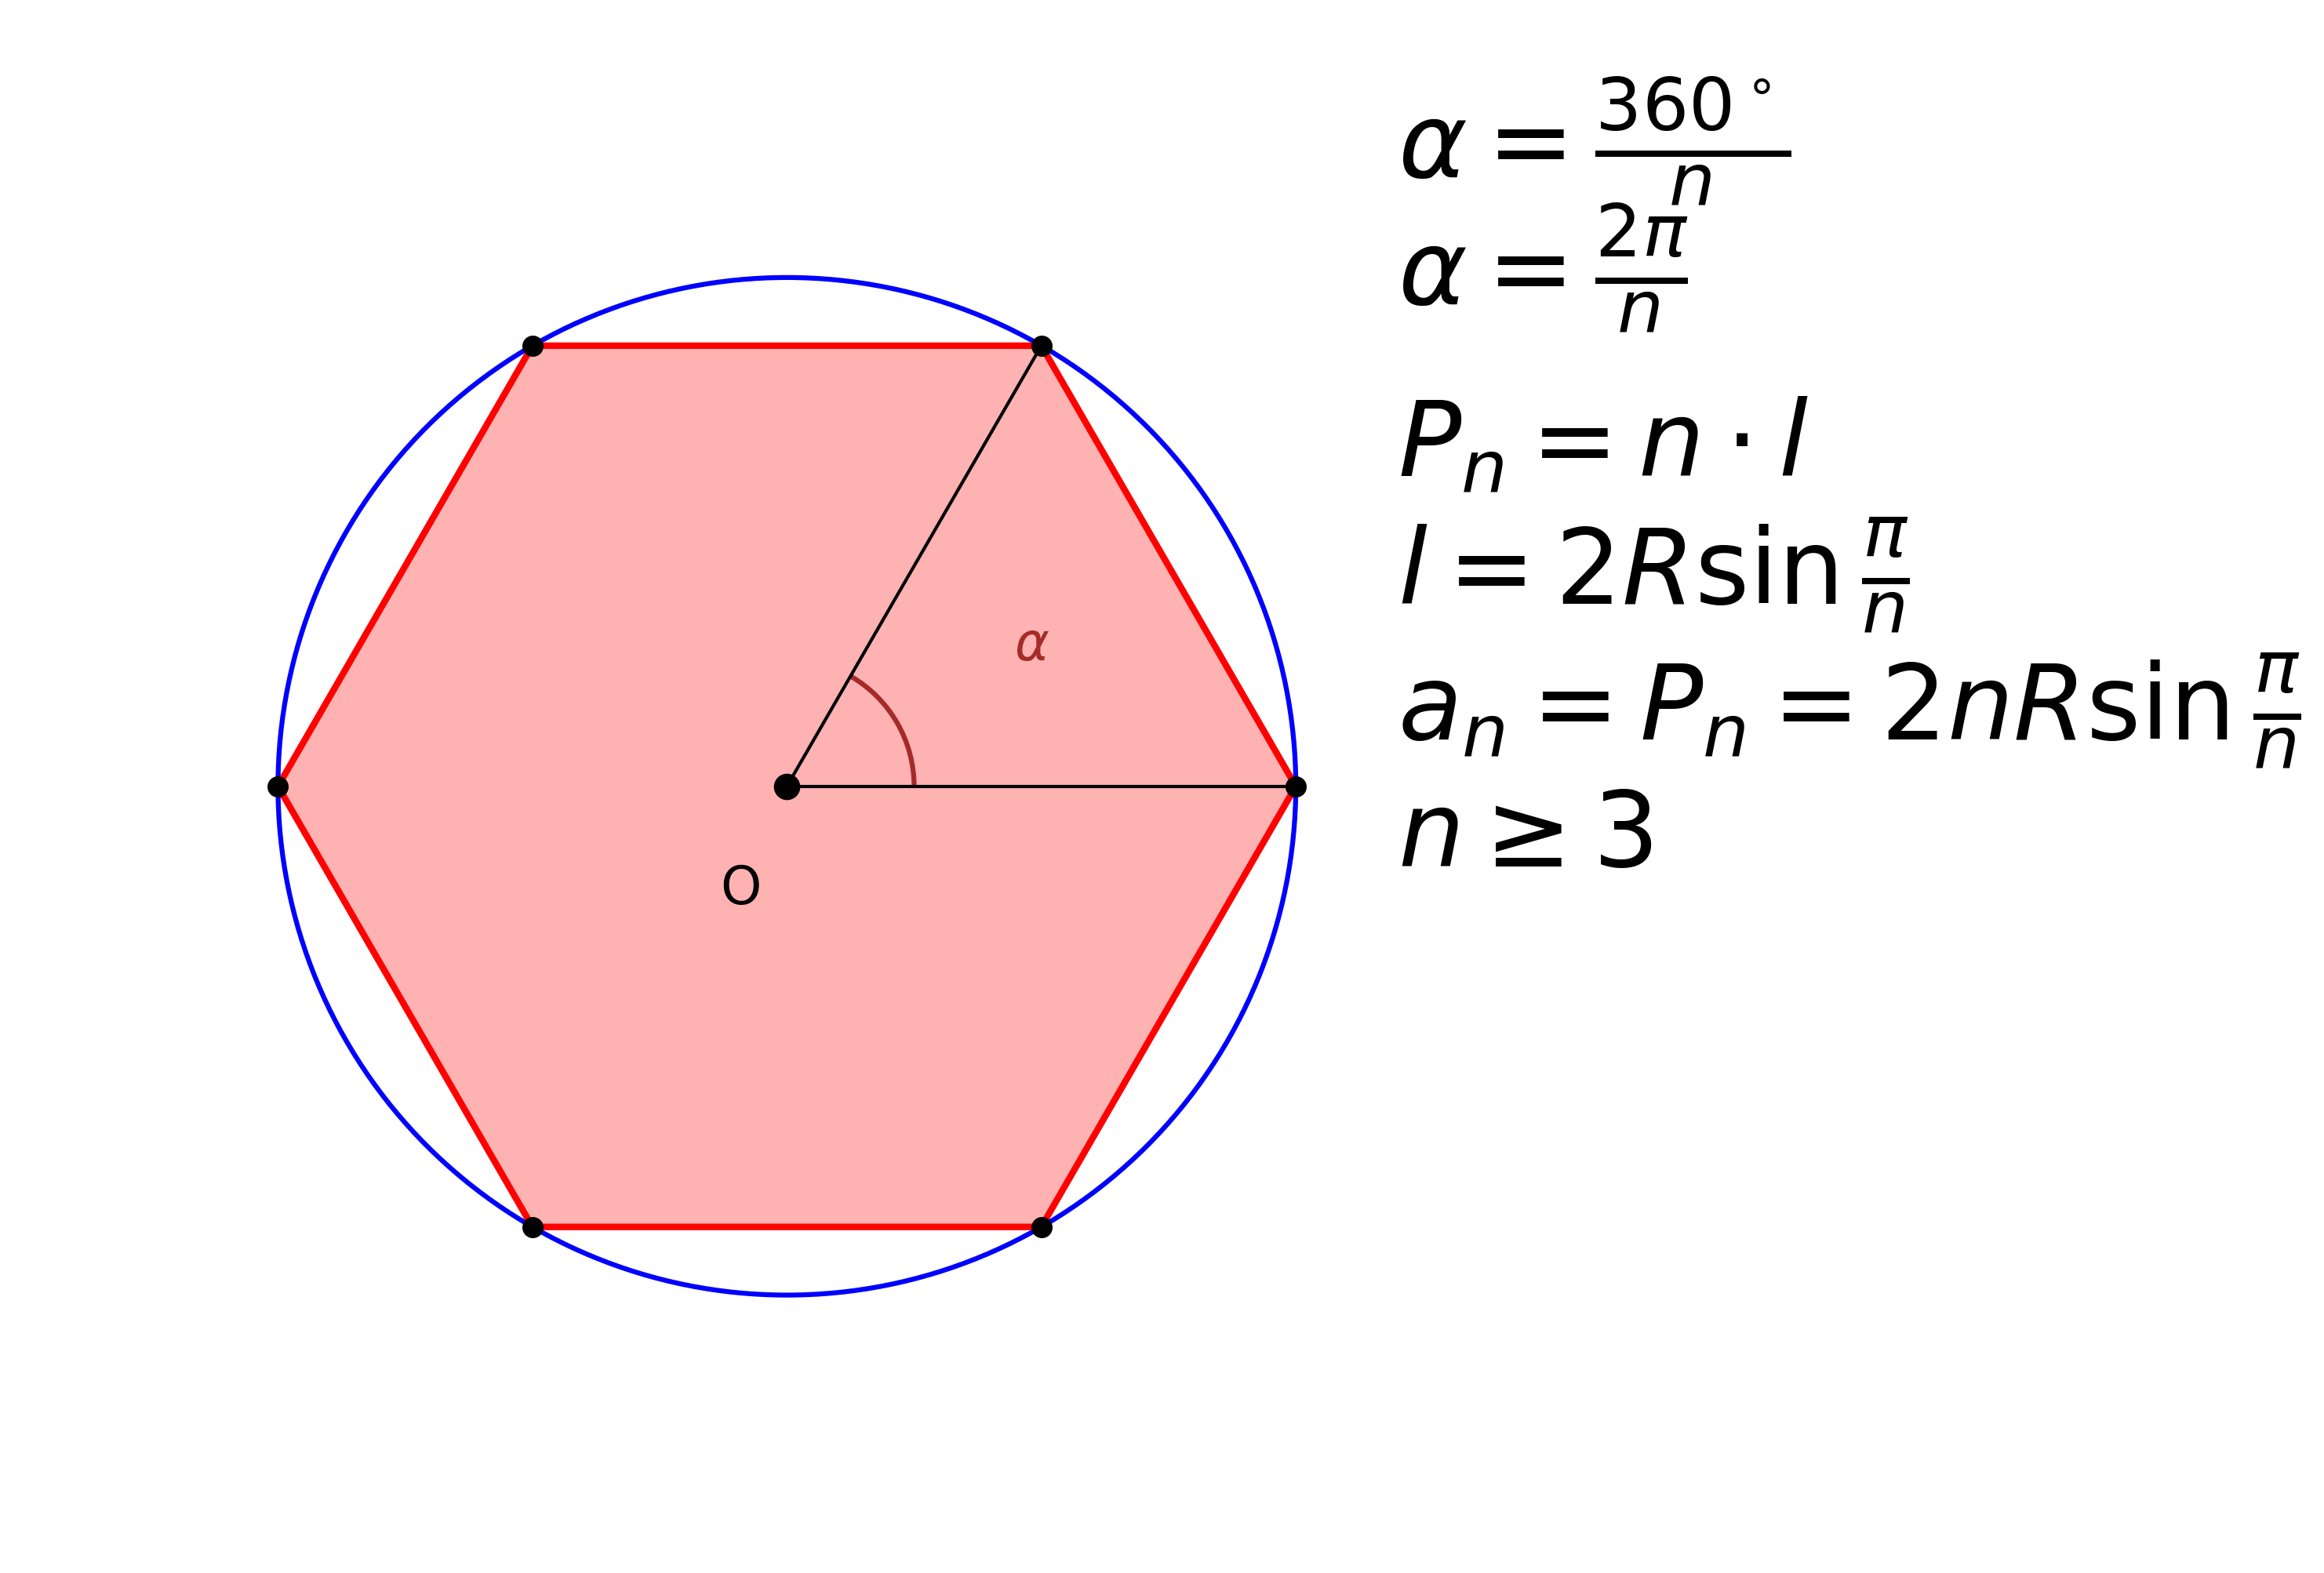
\includegraphics[width=0.5\textwidth]{img/n_gon_in_circle.png}%
    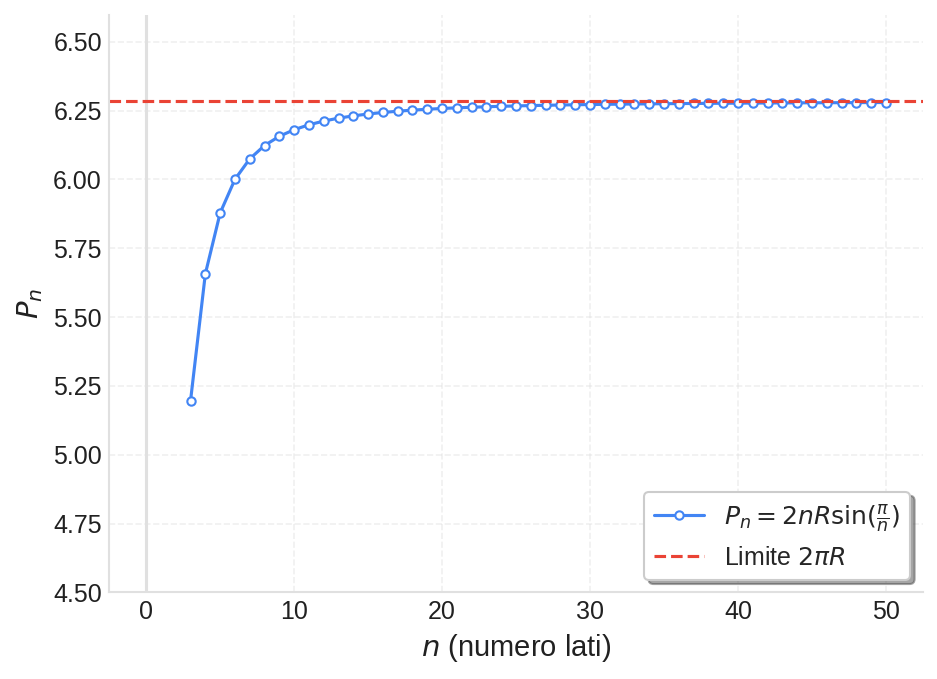
\includegraphics[width=0.5\textwidth]{img/esempio8_succ_numeriche.png}
\end{figure}
\[
\begin{aligned}
&P_{n}=n \cdot l\\
&\alpha = \frac{2\pi}{n} \\
&l=2R\sin \frac{\pi}{n} \\
&\boxed{a_{n}=P_{n}=2nR\sin \frac{\pi}{n}} \\
&n\geq3
\end{aligned}
\]

\section{Limiti di successioni}\label{limiti-di-successioni}
\begin{figure}[H]
    \centering
    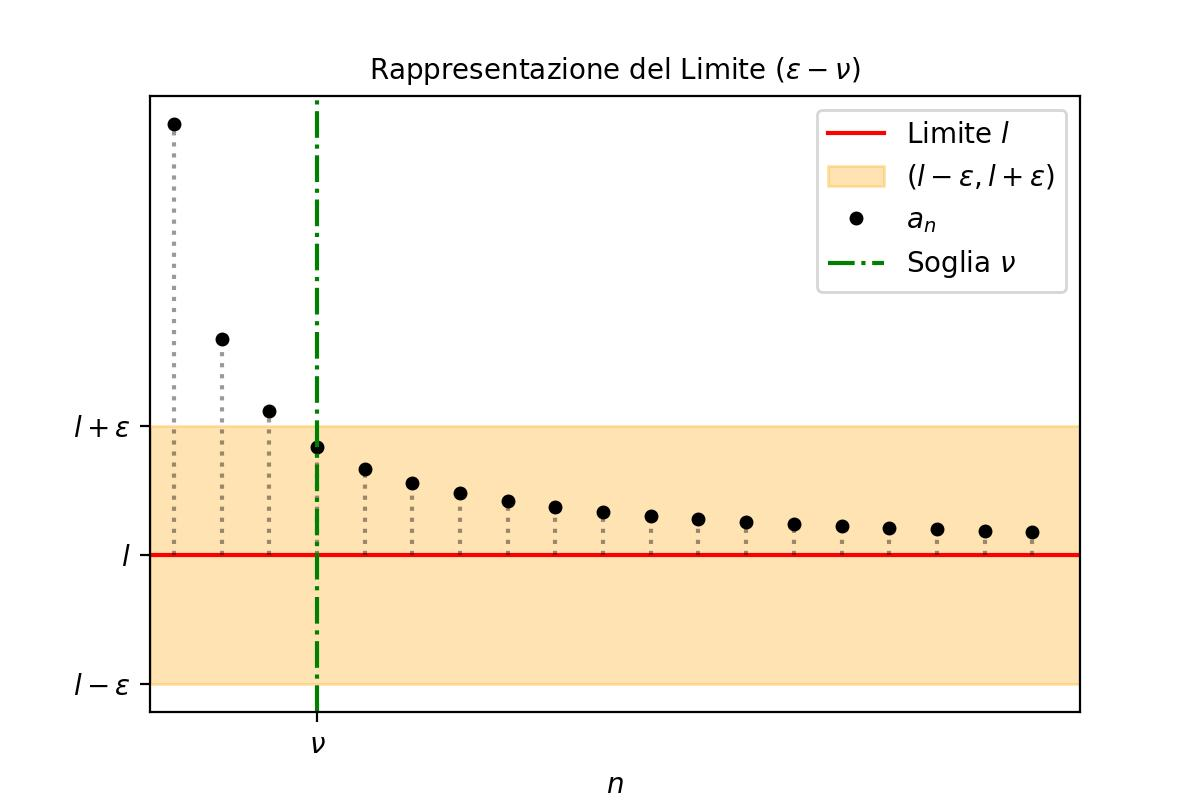
\includegraphics[width=0.8\textwidth]{img/lim_succ_num.png}
    \caption{Rappresentazione grafica del limite di una successione.}
\end{figure}

\defn{Limite di una successione numerica (Convergenza)}{
Assegnata una successione di termine generale $a_{n}$, diremo che $a_{n}$ tende ad $l\in \R$ o che $a_{n}$ converge ad $l\in \R$ se:
\[\forall\epsilon>0\exists \nu>0 :l-\epsilon<a_{n}<l+\epsilon \;\forall n>\nu\]
equivale a dire che:
\[\forall\epsilon>0 \exists \nu>0:|a_{n}-l|<\epsilon \;\forall n > \nu\]
e scriveremo:
\[\boxed{\lim_{ n \to \infty } a_{n}=l}\]
(Posso omettere $+\infty$ nel limite).
\bigskip
(IN PAROLE POVERE):
\begin{itemize}
    \item $\epsilon$ è la larghezza dell'imbuto
    \item $\nu$ è la soglia
    \item $l-\epsilon<a_{n}<l+\epsilon$ è il filtro
\end{itemize}
}

Appunto scollegato:
(a volte con $\nu$)
$x>0,\; x \in \R$
$[x]=$ parte intera (funzione floor())

\newpage
\subsection{Esempi di Limiti di successioni}\label{esempi-limiti-di-successioni}

\ex{1 — Limite della successione $a_n = \frac{1}{n}$}
\begin{figure}[H]
    \centering
    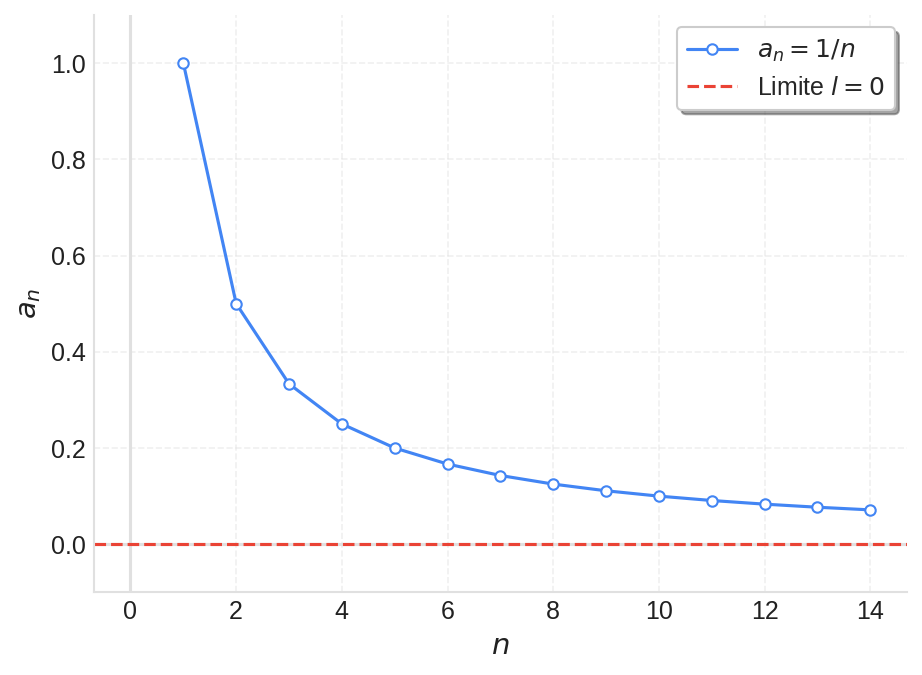
\includegraphics[width=0.8\textwidth]{img/successione_1-su-n.png}
    \caption{Successione $a_n = 1/n$.}
\end{figure}

\prop{
\[    
\lim_{n \to \infty} \frac{1}{n} = 0
\]
}

\pf{
Devo dimostrare che:
\[
\forall \, \epsilon > 0 \; \exists \, \nu > 0 \; \text{tale che} \; l - \epsilon < a_n < l + \epsilon \quad \forall n > \nu
\]
Nel nostro caso $l = 0$ e $a_n = \frac{1}{n}$, quindi la condizione diventa:
\[\boxed{-\epsilon < \frac{1}{n} < \epsilon}\]
Poiché $\frac{1}{n} > 0$ per ogni $n$, la disuguaglianza di sinistra è sempre vera.
\par
Rimane quindi da imporre:
\[
\frac{1}{n} < \epsilon
\]
da cui segue:
\[
n > \frac{1}{\epsilon}
\]
Poniamo quindi:
\[
\nu = \frac{1}{\epsilon}
\]
Allora, per ogni $n > \nu$, risulta verificata la disuguaglianza \par
\[
-\epsilon < \frac{1}{n} < \epsilon
\]
per ogni $\epsilon > 0$.
\par
Quindi:
\[
\boxed{\lim_{n} \frac{1}{n} = 0}
\]
}

\subsection{Successioni Convergenti o Infinitesime}\label{successioni-convergenti-o-infinitesime}

\defn{Definizione}{
Se $a_{n}$ tende ad $l \in \R$ scriviamo anche che: $a_{n}\to l\in \R$
\begin{itemize}
    \item Se $a_{n}\to l\in\R$ diremo che la successione è \textbf{Convergente}.
    \item Se $l=0$ diremo che è \textbf{Infinitesima}.
\end{itemize}
(Non completa tutti i casi):
}

\ex{3: $a_n = n$}
\[a_n = n\]
\begin{figure}[H]
    \centering
    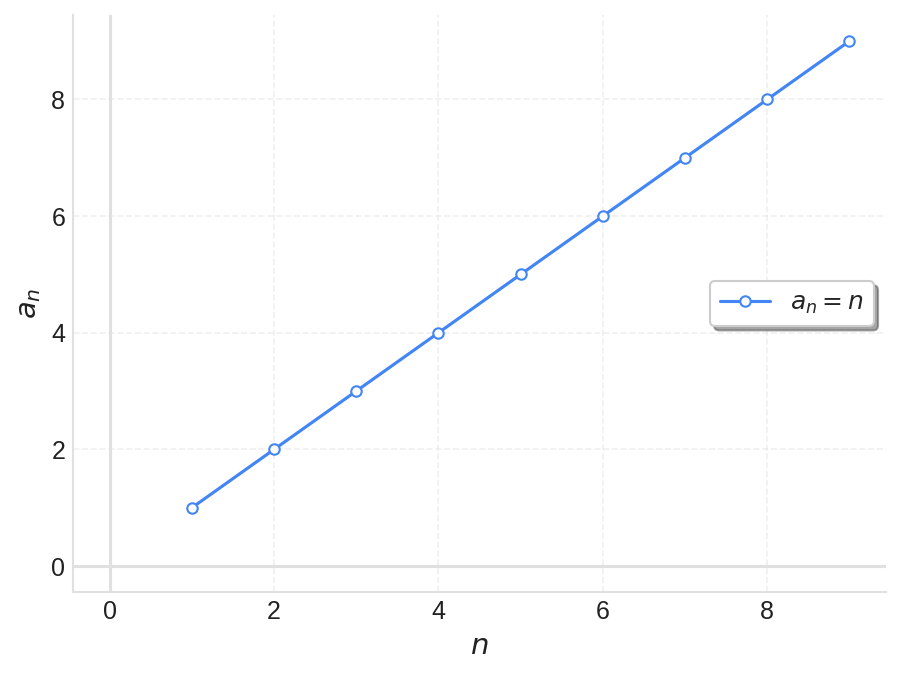
\includegraphics[width=0.6\textwidth]{img/succ_a_n=n.png}
    \caption{Successione $a_n=n$.}
\end{figure}

\subsection{Successioni Divergenti}\label{successioni-divergenti}

\defn{Definizione divergenza a $\infty$}{
Assegnata una succesione $a_{n}$ diremo che $a_{n}$ diverge \textbf{POSITIVAMENTE} oppure che diverge o tende a $+\infty$ se:
\[\boxed{\forall M >0 \; \exists \nu >0 : a_{n}>M \quad \forall n>\nu}\]
e scriveremo che:
\[\lim_{ n \to \infty } a_{n}=+\infty \quad\text{ oppure che }\quad a_{n}\to + \infty\]
Diremo che $a_n$ diverge \textbf{NEGATIVAMENTE} oppure che diverge o tende a $-\infty$ se:
\[\boxed{\forall M >0 \; \exists \nu >0 : a_{n}<-M \quad \forall n>\nu}\]
e scriveremo che:
\[\lim_{ n \to \infty } a_{n}=-\infty \quad\text{ oppure che }\quad a_{n}\to - \infty\]
}

\subsection{Successioni regolari o irregolari}\label{successioni-regolari-o-irregolari}

\ex{2 - Successione oscillante $a_n = (-1)^n$}
\begin{figure}[H]
    \centering
    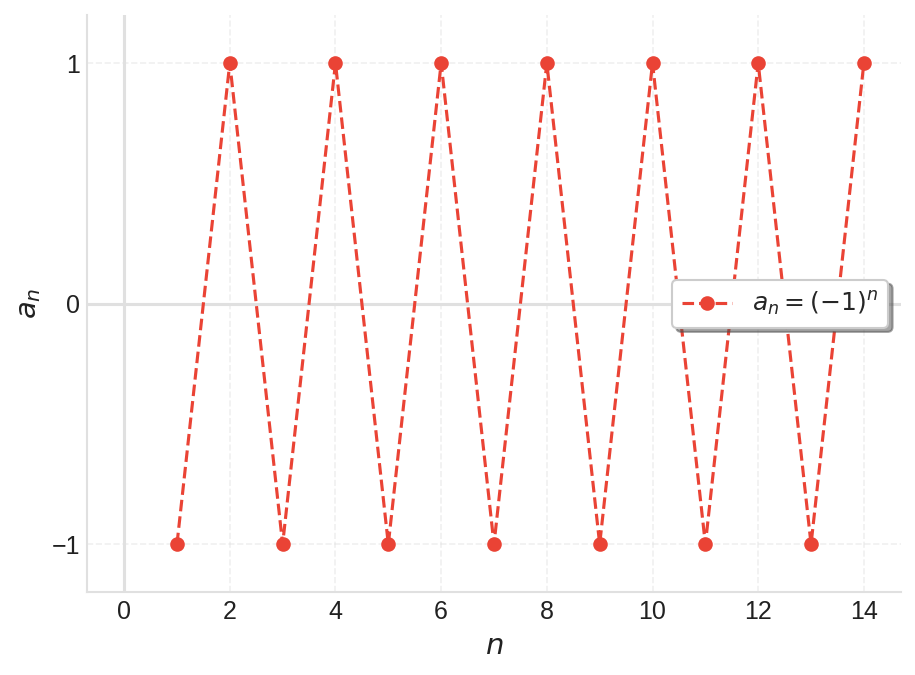
\includegraphics[width=0.6\textwidth]{img/succ_osc_1_-1.png}
    \caption{Successione oscillante $a_n = (-1)^n$.}
\end{figure}
Immaginate, per assurdo, che la successione
\[a_n = (-1)^n\]
ammetta un limite.
Allora il limite dovrebbe essere contemporaneamente $1$ (per i termini pari) e $-1$ (per i termini dispari), il che è impossibile.
Quindi:
\begin{itemize}
    \item La successione \textbf{non è convergente}.
    \item Non diverge a $+\infty$ né a $-\infty$.
    \item Questa successione è detta \textbf{irregolare} o \textbf{oscillante}.
\end{itemize}

\defn{Definizione (successione irregolare / oscillante)}{
Sia $a_n$ una successione numerica:
\begin{itemize}
    \item Se $a_n$ \textbf{ammette il limite}, è \textbf{convergente} o \textbf{regolare}.
    \item Se $a_n$ \textbf{non ammette limite} (né finito né infinito), è \textbf{irregolare} o \textbf{oscillante}.
\end{itemize}
}

\section{Definizione di Intorno}

\defn{Intorno}{
Sia $l \in \R$. Si chiama \textbf{intorno di $l$} qualsiasi intervallo aperto di $\R$ contenente $l$.
\textbf{Esempio:} l'intervallo aperto $]1,\frac{5}{2}[$ è un intorno di $2$.

Un \textbf{intorno di $+\infty$} è, per definizione, una semiretta dx aperta:
\textbf{Esempio:} $]2,+\infty[$.
Analogamente, un \textbf{intorno di $-\infty$} è una semiretta sx aperta:
\textbf{Esempio:} $]-\infty, 2[$.
Gli intorni si possono indicare anche come $I(l)$, $I(+\infty)$, $I(-\infty)$.
}

\prop{
Sia $a_n$ una successione numerica.
Allora:
\[
\lim_{n \to \infty} a_n = l \in \overline{\R}
\quad \iff \quad
\forall\, I(l)\; \exists\, \nu \in \N : a_n \in I(l) \quad \forall n > \nu.
\]
}


\pf{
La dimostrazione segue direttamente dalla definizione di limite ed è quindi ovvia.
}

\section{Teorema di Unicità del Limite}\label{teorema-unicita-limite}

\defn{Teorema di Unicità del Limite}{
Ogni successione regolare ammette \textbf{UNO e UN SOLO limite}.
}

\pf{
Si procede per assurdo: \par
Supponiamo che:
\begin{itemize}
    \item $a_n \to l_1 \in \overline{\R}$
    \item $a_n \to l_2 \in \overline{\R}$
\end{itemize}
con $l_1 \neq l_2$.
Essendo $\R$ un campo ordinato, supponiamo senza perdita di generalità che $l_1 < l_2$.
\begin{figure}[H]
    \centering
    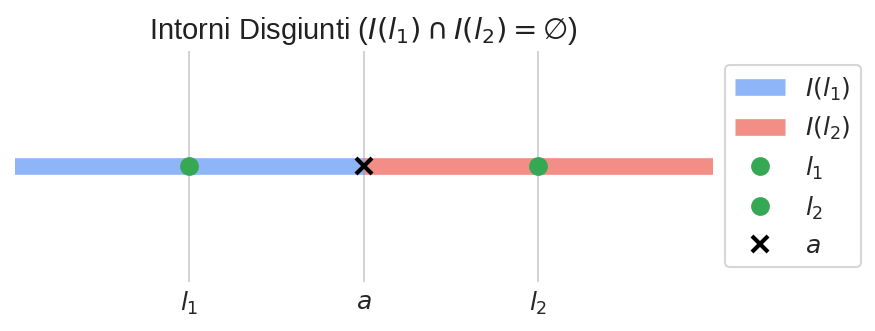
\includegraphics[width=0.8\textwidth]{img/intervalli_unicita_lim.png}
    \caption{Intervalli disgiunti per la dimostrazione per assurdo.}
\end{figure}

Poiché $l_1 < l_2$, esiste $a \in \R$ tale che $l_1 < a < l_2$.
Consideriamo gli intorni disgiunti:
\[I(l_1) = ]-\infty, a[, \quad I(l_2) = ]a, +\infty[\]
L'intersezione tra questi due intorni è ovviamente vuota:
\[I(l_1) \cap I(l_2) = \varnothing\]

Per ipotesi, $a_n \to l_1$, allora per questo intorno $I(l_1)$:
\[\exists \, \nu_1 \in \N \; : \; a_n \in I(l_1) \quad \forall n > \nu_1\]
Analogamente, $a_n \to l_2$ allora per questo intorno $I(l_2)$:
\[\exists \, \nu_2 \in \N \; : \; a_n \in I(l_2) \quad \forall n > \nu_2\]

Poniamo:
\[\nu = \max(\nu_1, \nu_2)\]
Allora $\forall n > \nu$, dovremmo avere:
\[a_n \in I(l_1) \cap I(l_2)\]
Ma $I(l_1) \cap I(l_2) = \varnothing$, ASSURDO.
Quindi la nostra ipotesi iniziale era falsa e il limite, se esiste, è \textbf{unico}.
}

\section{Proprietà delle successioni numeriche}

\defn{Successione Limitata}{
Sia assegnata una successione $a_n$ diremo che è:
\begin{itemize}
    \item \textbf{superiormente limitata} se:
    \[\exists B \in \R : a_n \leq B \quad \forall n \in \N\]
    \item \textbf{inferiormente limitata} se:
    \[\exists A \in \R : A \leq a_n \quad \forall n \in \N\]
    \item \textbf{limitata} se lo è sia inferiormente che superiormente.
\end{itemize}
In quest'ultimo caso:
\[\boxed{A\leq a_n \leq B} \quad \text{oppure} \quad | a_n | \leq M \quad \forall n \in \N\]
}

\rmkb{Osservazione:
Una successione Limitata non per forza converge!!
\ex{$(-1)^n$}
$(-1)^n$ è limitata ma oscillante.
}

\prop{
\textbf{Proposizione 1 (Convergenza $\implies$ Limitatezza)} \\
Sia $a_n$ una successione \textbf{convergente}, allora $a_n$ è \textbf{limitata}.
\[
(a_n \text{ convergente } \implies a_n \text{ limitata}) \quad \not\implies \quad
(a_n \text{ limitata } \implies a_n \text{ convergente})
\]
}


\pf{
Poichè $a_n \to l \in \R$ per ipotesi, allora $\forall \epsilon > 0 \exists \nu > 0$ tale che:
\[\boxed{l-\epsilon < a_n < l + \epsilon \qquad \forall n > \nu}\]
Sia $\epsilon = 1 \implies \exists \nu > 0:$
\[l-1 < a_n < l +1 \quad \forall n > \nu\]
Ma a noi serve $\forall n \in \N$.
Allora:
\[
E = \{a_1, a_2, a_3, \dots , a_{\lfloor\nu\rfloor}, l-1, l+1 \}
\]
Sia $A = \min E$ e $B = \max E$.
Allora:
\[A \leq a_n \leq B \quad \forall n \in \N\]
}

\prop{
\textbf{Proposizione 2 (Divergenza positiva)} \\
Se $a_n \to +\infty$, allora la successione $a_n$ è \textbf{inferiormente limitata}.
}

\pf{
Per hp $a_n \to +\infty$ quindi:
\[\forall M>0 \; \exists \nu > 0 : a_n > M \; \forall n > \nu\]
Considero :
\[
E = \{a_1, a_2, a_3, \dots , a_{\lfloor\nu\rfloor}, M \}
\]
Sia $A = \min E$.
Allora per costruzione:
\[a_n \geq A \; \forall n \in \N\]
Ovvero è inferiormente limitata.
}

\prop{
\textbf{Proposizione 3 (Divergenza negativa)} \\
Se $a_n \to -\infty$, allora la successione $a_n$ è \textbf{superiormente limitata}.
\par
La dimostrazione è lasciata come \textbf{esercizio}.
}


\section{Successioni Monotone}

\defn{Definizione — Successioni Monotone}{
Diremo che una successione $a_n$ è:
\begin{itemize}
    \item \textbf{crescente} ($\nearrow$) se $a_n \leq a_{n+1} \quad \forall n \in \N$.
    \item \textbf{strettamente crescente} ($\nearrow_{S}$) se $a_n < a_{n+1} \quad \forall n \in \N$.
    \item \textbf{decrescente} ($\searrow$) se $a_n \geq a_{n+1} \quad \forall n \in \N$.
    \item \textbf{strettamente decrescente} ($\searrow_{S}$) se $a_n > a_{n+1} \quad \forall n \in \N$.
\end{itemize}
}

\ex{
\begin{itemize}
    \item $\frac{1}{n}\;\searrow_{S}$
    \item $n\;\nearrow_{S}$
    \item $\frac{(-1)^n}{n}$ NON è MONOTONA
    \item $2^n \nearrow_{S}$
    \item $a^n \qquad \searrow_{S} \text{ se } 0<a<1 \qquad \nearrow_{S} \text{ se } a>1$
\end{itemize}
}

\prop{
\textbf{Teorema di Regolarità delle Successioni Monotone} \\
Se $a_n$ è una successione \textbf{monotona}, allora $a_n$ è \textbf{regolare} (ammette limite finito o infinito).
}


\defn{Limite di Successioni Monotone}{
Sia $a_n$ una successione monotona. Allora:
\[
\lim_{n \to \infty} a_n =
\begin{cases}
\sup_n a_n & \text{se } a_n \text{ è crescente } (\nearrow) \\
\inf_n a_n & \text{se } a_n \text{ è decrescente } (\searrow)
\end{cases}
\]
}

\ex{
\begin{enumerate}
    \item $a_n = \arctan n$ \par
    $a_n \nearrow$, quindi
    \[
    \lim_{n} \arctan n = \sup a_n = \frac{\pi}{2}
    \]
    \item $a_n = \frac{1}{n}$ \par
    $a_n \searrow$, quindi
    \[
    \lim_{n} \frac{1}{n} = \inf a_n = 0
    \]
    \item $a_n = 2^n$ \par
    $a_n \nearrow$, quindi
    \[
    \lim_{n} 2^n = \sup a_n = +\infty
    \]
\end{enumerate}
}

\rmkb{Osservazione sulla Dimostrazione:
La dimostrazione si basa sulle proprietà di sup e inf e sull'assioma di completezza di $\R$.
}

\pf{
Per ipotesi $\boxed{a_{n}\leq a_{n+1}}\;\forall n$ e dobbiamo dimostrare che detto $l=\sup_{n} a_{n}$ allora $\lim_{n \to \infty} a_{n}=l$.
\par
DUE CASI:
\begin{enumerate}
    \item \textbf{Caso 1 ($l<+\infty$):}
    Dobbiamo dimostrare che:
    \[
    \boxed{\forall \epsilon >0 \exists \nu : l-\epsilon < a_{n} <l+\epsilon \quad \forall n > \nu }
    \]
    Sia $\epsilon$ fissato.
    Per la proprietà dell'estremo superiore, si ha che $\exists \nu \in \N$ tale che $l-\epsilon < a_{\nu}$.
    Poiché $a_n$ è crescente, per ogni $n > \nu$ si ha $a_n \geq a_\nu$.
    Inoltre, $l$ è l'estremo superiore, quindi $a_n \leq l$.
    Quindi, per $\forall n > \nu$:
    \[
    l-\epsilon < a_{\nu} \leq a_{n} \leq l < l+\epsilon \quad (\text{tesi})
    \]

    \item \textbf{Caso 2 ($l=+\infty$):}
    Dobbiamo dimostrare che:
    \[
    \boxed{\forall M > 0 \exists \nu > 0 : a_{n} > M \quad \forall n > \nu}
    \]
    Usiamo la proprietà del $\sup a_{n} = +\infty$: $\forall M > 0 \exists \nu \in \N$ tale che $a_{\nu} > M$.
    Poiché $a_n$ è crescente, $\forall n > \nu$ si ha $a_{n} \geq a_{\nu} > M$, da cui la tesi.
\end{enumerate}
La dimostrazione per $a_{n} \searrow$ è analoga.
}

\rmkb{Osservazione sulla Convergenza:
$a_{n}$ è monotona + limitata $\implies a_{n}$ convergente
}

\subsection{Proprietà definitivamente vera}

\defn{Definizione Proprietà Definitivamente Vera}{
Una proprietà che dipende da $n \in \N$ si dice \textbf{DEFINITIVAMENTE} vera se vale da un certo indice $n$ in poi.
}

\rmkb{Osservazione sulla Regolarità:
Nel Teorema di Regolarità, posso scrivere: "Se $a_n$ è una successione definitivamente \textbf{monotona}, allora $a_n$ è \textbf{regolare}."
}

\prop{
\textbf{Proposizione (Valore Assoluto)} \\
Se $a_n$ è una successione \textbf{convergente} e $a_n \to l$, allora vale:
\[
|a_n| \to |l|.
\]
}


\pf{
Si usa la disuguaglianza triangolare inversa: $|a-b|\geq ||a|-|b||$.
\[||a_{n}|-|l||< |a_{n} -l |<\epsilon \quad \forall n > \nu\]
}

\prop{
\textbf{Proposizione (Infinitesima)} \\
Si ha che:
\[
a_n \to 0 \quad \iff \quad |a_n| \to 0.
\]
}


% DA TERMINARE (? sul quaderno)



% Algebra dei Limiti

\section{Algebra dei Limiti}\label{algebra-de-limiti}

\subsection{Limiti Fondamentali}

\[
\lim_{n \to +\infty} n^{\alpha} = 
\begin{cases}
+\infty \quad \alpha>0\\ 
1 \quad \alpha=0\\ 
0 \quad \alpha<0
\end{cases}
\]

\[
\lim_{n \to +\infty} a^n = 
\begin{cases}
+\infty & a>1\\ 
1 & a=1\\ 
0 & 0<a<1
\end{cases}
\]

\[
\lim_{n \to +\infty} \log_a n = 
\begin{cases}
+\infty \quad a>1\\
-\infty \quad 0<a<1
\end{cases}
\]

Vogliamo sostituire \(a_n\) ad \(n\) per generalizzare.
\subsection{Proprietà (Limiti Finiti)}\label{proprieta-limiti-finiti}

Siano \(a_n\) e \(b_n\) due successioni \textbf{convergenti} tali che:  
\[a_n \to a \in \mathbb{R}, \quad b_n \to b \in \mathbb{R}\]

Allora valgono le seguenti proprietà:
\subsubsection{1. Somma e differenza}
\[
\lim_{n \to +\infty} (a_n \pm b_n) = a \pm b
\]
Dimostrazione: si utilizza la \textbf{disuguaglianza triangolare}.

\pf{
\begin{align} % Cambiato align in align per evitare numero equazione
 & |(a_{n}+b_{n})-(a+b)| = |(a_{n}-a)+(b_{n}-b)|\\
 & |(a_{n}-a)+(b_{n}-b)| \leq |a_{n}-a| + |b_{n}-b|
 \\
 & \text{Per ipotesi: } |a_{n}-a| < \frac{\epsilon}{2} \; \forall n>\nu_{1}, \quad |b_{n}-b| < \frac{\epsilon}{2} \;
 \forall n>\nu_{2} \\
 & \text{Sia } \nu = \max{\nu_{1},\nu_{2}}, \text{ Allora } \forall n>\nu \\
 & |(a_{n}+b_{n})-(a+b)| \leq |a_{n}-a|
 + |b_{n}-b| < \frac{\epsilon}{2} + \frac{\epsilon}{2} = \epsilon \\
 & \text{QUINDI: } \\
 & \forall \epsilon > 0, \; \exists \nu : |(a_{n}+b_{n})-(a+b)| < \epsilon \forall n> \nu
\end{align}
}

\subsubsection{2. Prodotto}\label{prodotto}
\[
   \lim_{n \to +\infty} (a_n \cdot b_n) = a \cdot b
\]

\subsubsection{3. Rapporto}\label{rapporto}
\[
   \lim_{n \to +\infty} \frac{a_n}{b_n} = \frac{a}{b}
\]
a patto che \(b_n \neq 0\) e \(b \neq 0\).

\subsubsection{4. Potenza}\label{potenza}
\[
   \lim_{n \to +\infty} (a_n)^{b_n} = a^{b}
\]
con \(a_n > 0\) (e quindi \(a > 0\)).\\
Tuttavia, \textbf{questa non è una condizione necessaria}: in alcuni
casi il limite può esistere anche se \(a \le 0\).
\subsubsection{Esempi}\label{esempi}

\ex{
\[\lim_{ n \to +\infty } \frac{n}{n+1}=\lim_{ n \to +\infty } \frac{n+1-1}{n+1}=\frac{n+1}{n+1} -\frac{1}{n+1}=\lim_{ n \to +\infty } 1 - \lim_{ n \to +\infty } \frac{1}{n+1} = 1- 0 = 1\]
}

\ex{
\[\lim_{ n \to +\infty } \frac{(-1)^n + \sqrt{n}}{n} = \lim_{ n \to +\infty } \frac{(-1)^n}{n} + \lim_{ n \to +\infty } \frac{\sqrt{n}}{n} = 0 + 0 = 0\]
}

\ex{
\[\lim_{n \to +\infty} \frac{n^2 + 3n - 1}{2n - 3} = \lim_{n \to +\infty} \frac{n^2\left(1 + \frac{3}{n} - \frac{1}{n^2}\right)}{n\left(2 - \frac{3}{n}\right)} = \lim_{n \to +\infty} \frac{n\left(1 + \frac{3}{n} - \frac{1}{n^2}\right)}{2 - \frac{3}{n}} = +\infty\]
}

\subsection{Algebra dei limiti in \texorpdfstring{$\overline{\mathbb{R}}$}{R esteso}}\label{algebra-dei-limiti-versione-2}

\subsubsection{Somma e differenza}

Siano \(a_n\) e \(b_n\) due successioni tali che:
\[a_n \to a \in \overline{\mathbb{R}}, \quad b_n \to b \in \overline{\mathbb{R}}\]
Allora: \[
\lim_{n \to +\infty} (a_n \pm b_n) = a \pm b \;(\text{Fatta eccezione del caso}\; \infty-\infty)
\] e dove si sottintende che: 
\begin{align} % Cambiato align in align
& +\infty \pm b = +\infty \\
& -\infty \pm b = -\infty\\
& +\infty + +\infty = +\infty\\
& -\infty - \infty = -\infty
\end{align}

\paragraph{Esempi}\label{esempi-1}

\ex{
\[
\lim_{ n \to \infty } 2^n + n = +\infty
\] oppure \[
\lim_{ n \to \infty } 2^n +\frac{1}{n} = +\infty
\]
}

\ex{
\(a_{n}=n^2\) e \(b_{n}=n\)
\[\lim_{ n \to \infty } n^2 -n = n^2(1-\frac{1}{n})=\lim_{ n \to \infty } n^2 \cdot \lim_{ n \to \infty } (1-0) = +\infty\]

\(a_{n}=n+1\) e \(b_{n}=n\) \[\lim_{ n \to \infty } a_{n}-b_{n}=1\]
}

\subsubsection{Prodotto}

Siano \(a_n\) e \(b_n\) due successioni tali che:
\[a_n \to a \in \overline{\mathbb{R}}, \quad b_n \to b \in \overline{\mathbb{R}}\]
Allora: \[\lim_{ n \to \infty } a_{n}b_{n}=ab\] Fatta eccezione il caso
\(+\infty \cdot 0\) dove si sottintende \(\pm \infty \cdot a = \infty\)
con la regola dei segni e \(\pm\infty \cdot \pm\infty = \infty\) (con la
regola dei segni).
\prop{
Se \(a_n\) è limitata inferiormente e
\(b_n \to +\infty\) Allora \[\lim_{ n \to \infty } a_{n}b_{n}=+\infty\]

\paragraph{Esempio}
\(a_{n}=n\to +\infty\) e
\(b_{n} =\frac{{(-1)^n}}{n}\to 0\)
\[a_{n}b_{n} = (-1)^n =\text{Indeterminata}\]
}

\prop{
Sia \(a_{n}\) limitata e \(b_n\) infinitesima.
Allora \[\lim_{ n \to \infty } a_{n}b_{n}=0\]
}
\pf{
Sia \(a_n\) \textbf{limitata}.  
Ciò implica che:
\[
\exists M > 0 \; : \; |a_n| \leq M \quad \forall n \in \mathbb{N}
\]
Sia inoltre \(b_n \to 0\), cioè:
\[
\forall \varepsilon_0 > 0 \; \exists \nu > 0 \; : \; |b_n| < \varepsilon_0 \quad \forall n > \nu
\]
Vogliamo mostrare che \(a_n b_n \to 0\), ovvero:
\[
\forall \varepsilon > 0 \; \exists \nu_1 > 0 \; : \; |a_n b_n| < \varepsilon \quad \forall n > \nu_1
\]
Sia \(\varepsilon > 0\).
Scegliamo \(\varepsilon_0 = \frac{\varepsilon}{M}\). Dalla definizione di \(b_n \to 0\), esiste \(\nu\) tale che \(|b_n| < \varepsilon_0\) per \(n > \nu\).
Scegliendo \(\nu_1 = \nu\), abbiamo:
\[
|a_n b_n| = |a_n| \cdot |b_n| < M \cdot \varepsilon_0 = M \cdot \left(\frac{\varepsilon}{M}\right) = \varepsilon \quad \forall n > \nu_1
\]
Quindi \(a_n b_n \to 0\).
}

\subsection{Forme indeterminate}\label{forme-indeterminate}
\begin{itemize}
\item
  \(\infty-\infty\)
\item
  \(\infty \cdot 0\)
\end{itemize}

\subsection{Esempi finali}\label{esempi-finali}

\ex{
\[\lim_{n \to \infty} \frac{n^2 + \sqrt{n} - 2(-1)^n + \arctan(n)}{n^3 - 1 + n^2 \cos(n) - n \sin(n)} = 0\]
}

\ex{
\[\lim_{n \to \infty} \frac{n^2 - 3\sqrt{n} + (-1)^n - 2 n^2 \arctan(n)}{\sqrt{n} - 3n + n^2} = 1-\pi\]
}

\ex{
\[\lim_{n \to \infty} \left( \arctan(-n) + \frac{3 \sqrt{n} \sin(n)}{\sqrt[3]{n^2 + 1}} + \frac{\pi n + (-1)^n}{n+1} \right) =\]
\[=\lim_{n \to \infty} \arctan(-n) + \lim_{n \to \infty} \frac{3 \sqrt{n} \sin(n)}{\sqrt[3]{n^2 + 1}} + \lim_{n \to \infty} \frac{\pi n + (-1)^n}{n+1}=\]
\[= 
 -\frac{\pi}{2} + 0 + \pi = \frac{\pi}{2}\]
}

% --- Inizio contenuti da "Algebra dei Limiti in R.md" ---

\subsection{Quoziente (in \texorpdfstring{$\overline{\mathbb R}$}{R esteso})}

\prop{
Sia \(b_n \to \pm \infty\) allora \(\boxed{\frac{1}{b_n} \to 0}\)
}
\pf{
Supponiamo che \(b_n \to +\infty \implies\)
\[\forall M > 0 \; \exists \nu > 0 : \boxed{b_n > M \; \forall n > \nu}\]
Per dimostrare la proposizione devo dimostrare che:
\[\forall \epsilon > 0 \; \exists \nu' > 0 : \frac{1}{|b_n|}<\epsilon \; \forall n > \nu' \]
Scegliendo \(M = 1/\epsilon\), dall'ipotesi \(\exists \nu\) tale che \(\forall n > \nu\)
\[ b_n > M = \frac{1}{\epsilon} \]
Essendo \(b_n\) e \(\epsilon\) positivi (definitivamente),
\[ 0 < \frac{1}{b_n} < \epsilon \]
Quindi \(\left|\frac{1}{b_n}\right| < \epsilon\) scegliendo \(\nu' = \nu\).
Quindi \(\frac{1}{\infty} = 0\) (IMPORTANTE!!!)
}

\prop{
Sia \(b_{n}\to 0\)
}
\pf{
Se
\(b_{n}\to 0 \implies \forall \epsilon > 0 \; \exists \nu > 0 :|b_{n}|<\epsilon \quad \forall n>\nu\)
\[\forall M > 0 \; \exists \nu'>0 : \begin{cases}
\frac{1}{b_{n}}>M \forall n>\nu' \quad \left( \frac{1}{b_n}\to +\infty \right)\\
\frac{1}{b_{n}}<-M \forall n>\nu' \quad \left( \frac{1}{b_n}\to -\infty \right)
\end{cases}\] Non posso dire qual è il caso.
}

\prop{
Sia \(b_{n}\to 0\) e definitivamente
\textbf{positiva} \(\implies \frac{1}{b_{n}}\to +\infty\)

Sia \(b_{n}\to 0\) e definitivamente \textbf{negativa}
\(\implies \frac{1}{b_{n}}\to -\infty\)

Se \(b_{n}\to 0\) e definitivamente positiva:
\[\exists \nu_{1}:b_{n}>0 \;\forall n > \nu_{1}\] 
In sintesi: \[b_{n}\to 0^+\]
}

\rmkb{
\subsubsection*{Convenzioni sul Quoziente}
\begin{align} % Cambiato align in align
 & \frac{1}{\infty}=0\\
 & \frac{1}{0^+}=+\infty \\
 & \frac{1}{0^-}=-\infty
\end{align}
}

\prop{
Siano
\(a_{n}\to a \in \overline{\mathbb{R}}, b_{n}\to b \in \overline{\mathbb{R}}\)

Allora: \[\frac{a_{n}}{b_{n}}=\frac{a}{b}\] secondo le convenzioni
adottate ad eccezzione dei casi \(\frac{\infty}{\infty}\)
}

\subsection{Nuova forma indeterminata}
Da \(0 \cdot \infty\):
\begin{itemize}
\item \(\frac{\infty}{\infty}\)
\item \(\frac{0}{0}\)
\end{itemize}

\subsection{Esponenziale}

\prop{
Sia \(a>1\) e sia
\(a_n \to l \in \overline{\mathbb R}\)

Allora: \[
\lim_{n \to +\infty} a^{a_n} = 
\begin{cases}
a^l &l \in \mathbb{R}\\
+\infty &l=+\infty\\
0 &l=-\infty
\end{cases}
\]
}

\rmkb{
\subsubsection*{Convenzioni su Esponenziali e Logaritmi}
\paragraph{Caso \(a>1\):}
\begin{align} % Cambiato align in align
    a^{+\infty} = + \infty \quad & \quad a^{-\infty} = 0 \\
    \log_a (+\infty) = +\infty \quad & \quad \log_a (0^+) = -\infty
\end{align}
\paragraph{Caso \(0<a<1\):}
\begin{align} % Cambiato align in align
    a^{+\infty} = 0 \quad & \quad a^{-\infty} = +\infty \\
    \log_a (+\infty) = -\infty \quad & \quad \log_a (0^+) = +\infty
\end{align}
}

\subsection{Forma generale degli esponenziali}
\[
{a_n}^{b_n} = e^{b_n \log {a_n}} \quad \text{ se } a_n > 0
\]

\prop{
\[
{a_n}^{b_n} \to
\begin{cases}
a^b \text{ se } a \in ] 0, +\infty [ \text{ e } 
b \in \mathbb{R}\\
\uparrow \text{TRANNE F.I. : } (e^{b \log a} \text{ con } b \log a = 0 \cdot \infty)
\end{cases}
\]
}

\subsection{Nuove F.I.}
\begin{itemize}
\item
  \(\infty^0\)
\end{itemize}

\ex{
\[e^{\log a_{n}}=e^{0 \cdot \infty} = a_{n}^{b_{n}}=+\infty^0\]
}

\prop{
Se \(a_n>0\) e \(a>0\) allora
\(a_{n}^{b_{n}} \to a^b\) con le convenzioni adottate tranne:
\[\infty^0 \qquad 1^\infty \qquad 0^0\]
}

\rmkb{
\subsubsection*{Riepilogo: Algebra Estesa dei Limiti (\(\overline{\mathbb{R}}\))}
\paragraph{Rapporti}
\begin{align} % Cambiato align in align
& \frac{1}{\infty}=0 \\
& \frac{1}{0^+}=+\infty \\
& \frac{1}{0^-}=-\infty
\end{align}

\paragraph{Esponenziali}
Caso \(a>1\): 
\begin{align} % Cambiato align in align
& a^{+\infty} = + \infty \\
& a^{-\infty} = 0
\end{align}
Caso \(0<a<1\): 
\begin{align} % Cambiato align in align
& a^{+\infty} = 0 \\
& a^{-\infty} = +\infty
\end{align}

\paragraph{Logaritmi}
Caso \(a>1\): \[
\log_a (+\infty) = +\infty
\] Caso \(0<a<1\): \[
\log_a (+\infty) = -\infty
\]
}

% ==================================================
% INIZIO CONTENUTO AGGIUNTO
% ==================================================

\section{Teorema del confronto (Teorema dei carabinieri)}\label{teorema-del-confronto-teorema-dei-carabinieri}

\defn{Teorema del confronto}{
Valgono le seguenti affermazioni:
\begin{enumerate}
    \item Siano \(a_{n},b_{n},c_{n}\) tali che
    \[a_{n}\geq b_{n}\geq c_{n} \quad \forall n \in \mathbb{N}\]
    se \(a_{n}\to l \in \mathbb{R}\) e
    \(c_{n}\to l \in \mathbb{R} \implies b_{n}\to l\)
    \item Se \(a_{n}\leq b_{n} \quad \forall n \in \mathbb{N}\) e
    \(a_{n}\to +\infty\) allora \(b_{n}\to +\infty\)
    \item Se \(a_{n}\leq b_{n} \quad \forall n \in \mathbb{N}\) e
    \(b_{n}\to -\infty\) allora \(a_{n}\to -\infty\)
\end{enumerate}
}

\ex{
Posso calcolare:
\[\lim_{ n } n! = +\infty \]
perchè \(n! > n\)
}

\pf{
\textbf{(1)} Hp:
\begin{itemize}
    \item \(a_{n}\to l\in \mathbb{R}\)
    \item \(c_{n}\to l\in \mathbb{R}\)
    \item \(a_{n}\leq b_{n}\leq c_{n}\)
\end{itemize}
Per hp: \[
\begin{aligned}
& a_{n}\to l \in \mathbb{R} \implies \forall \epsilon > 0 \exists \nu_{1}>0: l- \epsilon <a_{n}<l+\epsilon \forall n> \nu_{1} \\
& c_{n}\to l \in \mathbb{R} \implies \forall \epsilon > 0 \exists \nu_{2}>0: l- \epsilon <c_{n}<l+\epsilon \forall n> \nu_{2} \\
& \forall n> \nu_{1} \;
l - \epsilon <a_{n}\leq b_{n} \leq c_{n} <l+\epsilon \; \forall n> \nu_{2} \implies \\
& l-\epsilon < b_{n} <l +\epsilon \;
\forall n > \nu = \max\{\nu_{1}, \nu_{2}\} \\
\end{aligned}
\]
}

\pf{
\textbf{(2)} Per hp: \(a_{n}\to +\infty\)
\[\forall M > 0 \exists \nu_{1}>0 : a_{n}> M \;
\forall n>\nu_{1}\] Th:
\(b_{n}\to +\infty\) ovvero:
\[\forall M > 0 \exists \nu>0 : b_{n}> M \;
\forall n> \nu\]

Per hp: \(b_{n}\geq a_{n}>M\) 
\begin{align} % Cambiato align in align
& \forall n \in \mathbb{N}\\
& \forall n>\nu_{1}\\
& \forall n > \nu_{2}\\ \\
& \text{Quindi } \forall n> \nu = \max\{\nu_{1}, \nu_{2}\}
\end{align}
}

\section{Continuità di Seno e Coseno}\label{continuita-di-seno-e-coseno}

\prop{
Sia \(a_{n}\to a \in \mathbb{R}\) allora:
\begin{itemize}
    \item \(\sin a_{n} \to \sin a\)
    \item \(\cos a_{n} \to \cos a\)
\end{itemize}
In particolare se \(a_{n}\to 0\) si ha: 
\begin{align} % Cambiato align in align
& \lim_{ n \to \infty } \sin a_{n} = 0 \\
& \lim_{ n \to \infty } \cos a_{n} = 1
\end{align}
}

\pf{
\textbf{(Continuità del Seno in 0)} \par
Sia \(a_{n}\to 0\). Th:
\[
\lim_{ n \to \infty } \sin a_{n}=0
\] Ricordiamo le disuguaglianze notevoli: 
\begin{align} % Cambiato align in align
& \text{Se } 0<x<\frac{\pi}{2}: \quad 0 < \sin x < x \\
& \text{Se } -\frac{\pi}{2}<x<0: \quad x < \sin x < 0 \\
& \text{Prendendo il valore assoluto in entrambi i casi:} \\
& \boxed{|\sin x| \le |x|} \quad \text{ per } x \in ]-\frac{\pi}{2}, \frac{\pi}{2}[
\end{align}
 Poiché \(a_n \to 0\), \(a_n\) è definitivamente in
\(]-\frac{\pi}{2}, \frac{\pi}{2}[\).
Allora possiamo applicare la
disuguaglianza e vale definitivamente: \(0 \le |\sin a_n | \le |a_n |\)

Dato che (per ipotesi) \(\lim_{n \to \infty} |a_n| = 0\) e
\(\lim_{n \to \infty} 0 = 0\), per il Teorema del Confronto
(Carabinieri) anche la successione centrale converge a 0:
\[\lim_{n \to \infty} |\sin a_n| = 0\]
Questo implica
\(\lim_{n \to \infty} \sin a_n = 0\).
}

\pf{
\textbf{(Continuità del Seno in \(a \in \mathbb{R}\))} \par
Vogliamo dimostrare che se \(a_n \to a\), allora:
\[\lim_{n \to \infty} \sin a_n = \sin a\]

Definiamo una nuova successione \(b_n = a_n - a\).
Poiché \(a_n \to a\),
allora \(b_n \to 0\).

Riscriviamo \(a_n = b_n + a\) e usiamo la formula di addizione del seno:
\[\sin a_n = \sin(b_n + a) = \sin(b_n)\cos(a) + \cos(b_n)\sin(a)\]

Calcoliamo il limite di entrambi i membri (notando che \(\sin a\) e
\(\cos a\) sono costanti):
\[\lim_{n \to \infty} \sin a_n = \lim_{n \to \infty} \left( \sin(b_n)\cos(a) + \cos(b_n)\sin(a) \right)\]

Per l'algebra dei limiti:
\[\lim_{n \to \infty} \sin a_n = \left(\lim_{n \to \infty} \sin(b_n)\right) \cdot \cos(a) + \left(\lim_{n \to \infty} \cos(b_n)\right) \cdot \sin(a)\]

Poiché \(b_n \to 0\), usiamo i risultati già dimostrati per la
continuità in 0:
\begin{enumerate}
    \item \(\lim_{n \to \infty} \sin(b_n) = 0\)
    \item \(\lim_{n \to \infty} \cos(b_n) = 1\)
\end{enumerate}

Sostituendo questi limiti, otteniamo:
\[\lim_{n \to \infty} \sin a_n = (0) \cdot \cos(a) + (1) \cdot \sin(a) = \sin a\]

\emph{(Nota: La dimostrazione per \(\cos a_n \to \cos a\) è analoga,
usando la formula di addizione del coseno).}
}

\section{Limiti Notevoli Derivati}\label{limiti-notevoli}

\begin{enumerate}
\def\labelenumi{\arabic{enumi})}
%\tightlist % Rimosso comando non definito
\item
  Sia \(a>0\) allora:
\[\lim_{ n \to \infty } \sqrt[n]{ a }=1 \]
\textbf{Dimostrazione:}
Se \(a=1\) è ovvio.
Sia \(a>1\) consideriamo \(a_1=a\) e \(a_{2}=1=a_{3}=\dots=a_{n}\)
\begin{align} % Cambiato align in align
& G \leq A \implies \sqrt[n]{a} < \frac{a+n-1}{n} \text{Quindi }\\
& 1 < \sqrt[n]{a} < \frac{a+n-1}{n} \\
& \text{Se } 0<a<1: \\
& \sqrt[n]{a} = \left( \frac{1}{\sqrt[n]{a}} \right)^{-1}=\left( \sqrt[n]{\frac{1}{a}} \right)^{-1}\to 1 > \left( \sqrt[n]{\frac{1}{a}}\right)^{-1} > \frac{n}{a+n-1}
\end{align}

\item
  \[\lim_{ n \to \infty } \sqrt[n]n=1\]
  \textbf{Dimostrazione:}
  \begin{align} % Cambiato align in align
   & G\leq A \\
   & a_{1} = n \quad a_{2}=1=a_{3}=\dots=a_{n}\\
   & G = \sqrt[n] n < \frac{{n+n-1}}{n} \to \text{NO} \\
   & a_{1}=\sqrt n=a_{2} \quad a_{3}=\dots=a_{n}=1 \\
   & G = \sqrt[n] n < \frac{2\sqrt n + n -2}{n} = A
  \end{align}
\item
  \[\lim_{ n \to \infty } \sqrt[n]{ n^b }=1\] Perchè
  \((\sqrt[n]{ n})^b\) e se \(\sqrt[n]{n}=1\) Allora
  \((\sqrt[n]{ n})^b=1^b=1\)
\item
  Se \(a_{n}\to 0\) allora:
  \[\lim_{ n \to \infty } \frac{\sin a_{n}}{a_{n}} = 1 \text{ (ho rimosso l'altro limite che era sintatticamente errato)} \]
  %\[\lim_{ n \to \infty } \frac{\sin a_{n}}{n} = 1 \text{ anche } \lim_{ n \to \infty } \frac{n\sin_{1}}{n}=\frac{\sin{\frac{1}{n}}}{\frac{1}{n}}=1\]
  
\pf{
Sia x un angolo:
\begin{align} % Cambiato align in align
& \boxed{0<x<\frac{\pi}{2}} \\
& \sin x < x < \tan x = \frac{\sin x}{\cos x} \\ % Corretto: sin x < x < tan x
& 1< \frac{x}{\sin x} < \frac{1}{\cos x} \to \boxed{\cos x < \frac{\sin x}{x}<1} \implies \\
& \implies\text{ è pari quindi } \; |x|< \frac{\pi}{2} \\
& \text{Allora } \cos a_{n}< \frac{\sin a_{n}}{a_{n}} < 1 \\
 & \text{Calcolando il limite, sia a dx che a sx è 1.}
\end{align} 
}
\item
  Se \(a_{n}\to 0\) allora \[
  \lim_{ n \to \infty } \frac{\tan a_{n}}{a_{n}}=1
  \]
\pf{
\[ % Tolto > iniziale
 \lim_{ n \to \infty } \frac{\sin a_{n}}{\cos a_{n}} \cdot \frac{1}{a_{n}} = \lim_{ n \to \infty } \frac{\sin a_{n}}{a_{n}} \cdot \frac{1}{\cos a_{n}} = 1 \cdot 1 = 1
\]
}
\item
  Se \(a_{n}\to 0\) allora \[
  \lim_{ n \to \infty } \frac{1 - \cos a_{n}}{a_{n}} = 0
  \]
\pf{
(Usa dimostrazione del 7)
\[\lim_{ n \to \infty } \frac{1 - \cos a_{n}}{a_{n}} \cdot \frac{a_{n}}{a_{n}}=\lim_{ n \to \infty } \frac{1 - \cos a_{n}}{{a_{n}}^2} \cdot a_{n}= \frac{1}{2} \cdot 0 = 0\]
}
\item
  Se \(a_{n}\to 0\) allora \[
  \lim_{ n \to \infty } \frac{1- \cos a_{n}}{{a_{n}}^2}=\frac{1}{2}
  \]
\pf{
\begin{align} % Cambiato align in align
&\lim_{ n \to \infty }  \frac{1-\cos a_{n}}{{a_{n}}^2} \cdot\frac{1+\cos a_{n}}{1+\cos a_{n}} = \lim_{ n \to \infty } \frac{1-\cos^2 a_{n}}{{a_{n}}^2 (1 + \cos a_{n})}= \lim_{ n \to \infty } \frac{\sin^2 a_{n}}{{a_{n}}^2 (1 + \cos a_{n})} \\ % Corretto denominatore
& =  \lim_{ n \to \infty } \left( \frac{\sin a_{n}}{a_{n}} \right)^2 \cdot \frac{1}{1 + \cos a_{n}}=1^2 \cdot \frac{1}{1+1} = \frac{1}{2} % Corretto 1*1/2
\end{align}
}
\end{enumerate}

\subsection{Esempi}\label{esempi-limiti-notevoli-teo-confronto}

\ex{
\[\text{Se }a_{n}\to \frac{\pi}{2}^-\text{ allora: }\]
\[\lim_{ n \to \infty } \tan a_{n}= \frac{\sin a_{n}}{\cos a_{n}} = \frac{1}{0^+}= + \infty\]
}

\ex{
\[\text{Se }a_{n}\to \frac{\pi}{2}\text{ allora: }\]
\[\lim_{ n \to \infty } \tan a_{n}=\not \exists\]
}

\ex{
% Questo era già corretto
\begin{align} % Usato aligned invece di align dentro \[...\]
& \lim_{ n \to \infty } \frac{2n+{-1}^n + n^2 \sin\left( \frac{1}{n} \right)-\sqrt{n}}{\sqrt{ n }\arctan n -n + \sqrt{ n }\sin n+n \tan \left(\frac{1}{n}\right)} \\
& = \lim_{ n \to \infty } \frac{ n\left(2 + \frac{{-1}^n}{n} + n \sin\left( \frac{1}{n} \right) - \frac{1}{\sqrt{n}} \right)}{n\left( \frac{\arctan n}{\sqrt{n}} - 1 + \frac{\sin n}{\sqrt{n}} + \tan \left(\frac{1}{n}\right) \right)} \\
& = \frac{ 2 + 0 + 1 - 0 }{ 0 - 1 + 0 + 0 } = -3
\end{align}
}

\ex{
\begin{align} % Tolto \[...\] esterno
& \lim_{ n \to \infty } \frac{\log(n+1)-\log(n^3 - 2)- \sqrt[n]{ n+1 }}{\log n - 2 \log(n^2 -1) + (-1)^{n}} \\ 
& = \lim_{ n \to \infty } \frac{ \log\left(n\left(1 + \frac{1}{n}\right)\right) - \log\left(n^3\left(1 - \frac{2}{n^3}\right)\right) - \sqrt[n]{ n+1 } }{ \log n - 2 \log\left(n^2\left(1 - \frac{1}{n^2}\right)\right) + (-1)^{n} } \\ 
& = \lim_{ n \to \infty } \frac{ \left[\log n + \log\left(1 + \frac{1}{n}\right)\right] - \left[3\log n + \log\left(1 - \frac{2}{n^3}\right)\right] - \sqrt[n]{ n+1 } }{ \log n - 2 \left[2\log n + \log\left(1 - \frac{1}{n^2}\right)\right] + (-1)^{n} } \\ 
& = \lim_{ n \to \infty } \frac{ -2\log n + \log\left(1 + \frac{1}{n}\right) - \log\left(1 - \frac{2}{n^3}\right) - \sqrt[n]{ n+1 } }{ -3\log n - 2\log\left(1 - \frac{1}{n^2}\right) + (-1)^{n} } \\ 
& = \frac{-2}{-3} = \frac{2}{3}
\end{align}
}

\subsubsection{}\label{dimostrazione-esempio-precedente}

\ex{
Grazie al Teorema del confronto possiamo dimostrare
l'\hyperref[perim-pol-inscritto]{esempio 8 delle successioni
numeriche} 
\[
\lim_{ n \to \infty } P_{n} = 2Rn\sin \frac{\pi}{n}= \lim_{ n \to \infty } 2R n \frac{\sin \frac{\pi}{n}}{\frac{\pi}{n}} \frac{\pi}{n}= \lim_{ n \to \infty } 2R\pi \frac{\sin \frac{\pi}{n}}{\frac{\pi}{n}} = 2R\pi \cdot 1 = 2R\pi
\]
}
